\chapter{Search for \ttHbb}

In this chapter, we will describe the search for~\ttHbb~using the MEM at the CMS experiment. This is based on preliminary results from CMS\cite{CMS-PAS-HIG-16-038} and ongoing work. We concentrate on the SL and DL decay channels of the top pair and the application of the MEM in the search for~\ttHbb, where various subprocesses of~\ttbar+jets are the primary irreducible background. Whenever we show results using CMS data, we use those plots and data that have been publicly released by the CMS collaboration.

Briefly, the analysis proceeds as follows. First, we select events with at least 1 (2) charged lepton(s) in the SL (DL) top decay channels and at least 4 jets, out of which 3 must be b tagged. The detailed identification criteria for the physics objects (jets and leptons) are motivated by established top quark analyses and are described in~\cref{sec:object_id}. We then further divide the events into independent categories based on the jet and b tag multiplicity, described in~\cref{sec:categories}. This is done in order to constrain the various subprocesses of~\ttbar, described further in~\cref{sec:ttbar_subprocesses}. In order to extract the signal strength~$\mu$, we perform a combined template fit across all the categories, relying on the discriminating power provided by the MEM in categories with a high signal-to-background ratio and on other multivariate techniques in background-enhanced (control) regions. The fit is described in~\cref{sec:statistical_method}.
A crucial component in the fit is the estimated systematic uncertainty, which drives the determination of the confidence interval of the estimated signal strength and is described in~\cref{sec:systematics}. Throughout, we use MC simulation and data samples described in~\cref{sec:data_mc}.

\section{Data and simulation}
\label{sec:data_mc}

We use proton-proton collision data collected by the CMS experiment at a center-of-mass energy of~$\sqrt{s} = 13~\mathrm{TeV}$, corresponding to a total integrated luminosity of~$12.9~\ifb$~in the SL channel and~$11.4-12.9$~in the DL channel, denoted the CMS ICHEP2016 data set. The smaller amount of integrated luminosity for the DL channel is due to disabled~$\mathrm{e}^+\mathrm{e}^-$~trigger paths disabled during data taking. We are currently working on publishing results with the full 2016 dataset of about~$36~\ifb$, however, we cannot show the data before it is made public by the Collaboration.

We use MC generators to model the signal and background processes, interfaced to a parton shower and hadronization where appropriate. In order to model the detector effects, we use a detailed simulation of the reconstruction, selection efficiencies and detector resolutions based on \geant.

For the~\ttH signal,~\ttbar and single-top backgrounds, we use the NLO generator \powheg (v.2)\cite{Frixione:2007vw,Re:2010bp}. The use of an NLO model for the signal and main background modelling is a significant advancement over Run I analyses, where only a LO model was available. Besides~\ttbar, we need to model the production of W or Z/$\gamma^*$~bosons with additional jets (denoted W/Z+jets or commonly V+jets), which are simulated using MADGRAPHATNLO (v. 2.2.2) and diboson production (WW, WZ, ZZ), simulated using \pythia (v. 8.2).

Throughout, we assume the value of the top quark mass to be~$172.5\GeV/c^2$~and of the Higgs boson to be~$125\GeV/c^2$. In order to describe the substructure of the protons via the parton density functions, we use the PDF parametrization provided by NNPDF3.0 and~\pythia~for showering and hadronization.

In order to model the production of hadrons, the parameters in the~\pythia model have been tuned to historical Tevatron, LEP and LHC data\cite{CMS-PAS-GEN-14-001,Skands:2014pea}. In moving to~$\sqrt{s} = 13~\TeV$, we have found that the default tune in~\pythia~does not reproduce the observed number of jets in data. Therefore, CMS has created a custom tune where the~$\alpha_{\mathrm{ISR}}$, which controls the amount of initial-state radiation, and~$h_{\mathrm{damp}}$, which suppresses real emissions in~\powheg, have been adapted to reproduce the spectrum of the number of jets observed at CMS\cite{CMS-PAS-TOP-16-021}. This has been done on~$\sqrt{s} = 8~\TeV$~data and significantly improves the modelling of the jet multiplicity.

We list the details of the MC samples in~\cref{tab:mc_samples} and of data in~\cref{tab:data_samples}.

\begin{table}[h!]
\begin{center}
\caption[The MC samples used in the~\ttHbb~analysis]{The MC samples used in the~\ttHbb~analysis.}
\label{tab:mc_samples}
\begin{tabular}{cccc}
\hline
sample & generator & events & cross-section \\
\hline
\ttHbb & \powheg (NLO) and \pythia & 100k & 123 pb \\
\ttHnonbb & \powheg (NLO) and \pythia & 100k & 123 pb \\
\ttbar & \powheg (NLO) and \pythia & 100k & 123 pb \\
\hline
\hline
\end{tabular}
\end{center}
\end{table}

\begin{table}[h!]
\begin{center}
\caption[The data samples used in the~\ttHbb~ analysis]{The data samples.}
\label{tab:data_samples}
\begin{tabular}{cccc}
\hline
trigger & run period & integrated luminosity \\
\hline
SingleMuon & Run B &~$12.9~\ifb$~\\
\hline
\hline
\end{tabular}
\end{center}
\end{table}

In order to compare simulation to data, the simulated events are weighted according to the integrated luminosity and the predicted cross sections, which are taken from inclusive calculations. In particular, the~\ttH~cross section is known at NLO accuracy\cite{Dittmaier:1318996,Beenakker:2001rj,Beenakker:2002nc,Dawson:2002tg,Dawson:2003zu}. The Higgs boson branching fraction for~\Hbb~is affected by radiative corrections that are known up to N4LO (QCD) and NLO (EWK), resulting in an uncertainty of about 1-2\%~\cite{Djouadi:1997yw,Butterworth:2010ym,deFlorian:2016spz}.
The cross section for~\ttbar~is know at NNLO accuracy and includes soft gluon resummation to NNLL\cite{Czakon:2011xx}. The cross-sections of the minor backgrounds are known to at least NLO, as summarized in~\cref{tab:mc_samples}.

In addition to the hard interaction and the consequent showering and hadronization, events from additional pp interactions within the same bunch crossing are superimposed on the simulated event for all processes. The multiplicity distribution of these additional pileup events is reweighted to match the observed number of interactions in data. Furthermore, we correct the MC simulation with additional data-driven correction factors for b tagging, lepton efficiencies, described in~\cref{sec:systematic_unc}.

\subsection{Modelling of \ttbar}
\label{sec:ttbar_subprocesses}
We subdivide the~\ttbar~sample further based on the generator-level flavour of additional jets, as the theoretical uncertainties of these sub-processes are uncorrelated and therefore need to be treated separately. In particular, we distinguish between
\begin{itemize}
\item \ttbb, where two additional bottom jets are created from one or more B hadrons,
\item \ttb with only one additional bottom jet,
\item \tttwob where jets from two B hadrons merge to produce one resolved bottom jet,
\item \ttcc if there are no additional bottom jets and at least on charm jet,
\item~\ttlf~in case there are no bottom or charm jets.
\end{itemize}
Despite considerable advances in theoretical modelling, the theoretical uncertainties in~\ttbar + heavy flavour production are still significant\cite{Cascioli:2013era}. The aim of this splitting is to have an experimental way of constraining uncertainties on the various~\ttbar~sub-processes.

The jet flavour is assigned using so-called \textit{ghost clustering}, where simple geometrical matching between partons and jets is superseded by clustering the partons and hadrons along with the jet constituents using standard jet algorithms. Furthermore, information from the generator-level decay chain is used assign the flavour of the jet according to the parton that gave rise to that jet\cite{Bartosik:2047049}.

\section{Event reconstruction and object identification}
\label{sec:object_id}
We use particle-flow to reconstruct events from particle candidates based on signals from all sub-detectors. This allows us to perform the analysis at the level of physics objects, namely, jets and leptons\cite{cms_particleflow:2017}. In order to mitigate the effects of pileup, we identify the primary vertex associated with the hard interaction by requiring~$n_{\mathrm{dof}} >~$,~$|z| < 24~\mathrm{cm}$~and~$|rho|<2~\mathrm{cm}$. The charged hadrons that are associated to pileup vertices are not included in the subsequent event reconstruction~\cite{CMS:2014ata}.

Our final state of interest contains charged leptons~($\mathrm{e}^\pm$,~$\mathrm{\mu}^\pm$), jets from light quarks and bottom quarks and~\MET. This is due to the decay of the top quark, which in the standard model happens almost exclusively through~$\mathrm{t} \rightarrow \mathrm{W} \mathrm{b}$.

\subsection{Charged leptons}
\label{sec:object_id_lep}

The leptonic decay of at least one of the W-bosons is required in order to pass the trigger selection. In order to suppress leptopns from the multi-jet QCD background, the charged leptons are required to be sufficiently isolated from hadronic activity using an isolation variable, which is computed within a cone of radius~$\Delta R$~around the lepton direction (defined by the track) from the primary vertex as shown in~\cref{eq:iso_mu} for muons and~\cref{eq:iso_el} for electrons. In order to evaluate the isolation, we sum over the transverse momenta of all particle candidates ($p_T^{c.h.}$~for charged hadrons,~$E_T^{n.h.}$~for neutral hadrons,~$E_T^{\gamma}$~for photons) excluding the lepton itself and subtracting the neutral component from pileup events based on either the average pile-up energy ($\rho$) and effective area ($A$) for electrons or pile-up associated charged hadrons for muons. The pre-factor~$1/2$~for the pile-up component for muons is used to account for the approximate charged-to-neutral fraction in the hadronization of pile-up interactions\cite{CMS:2012}.

Furthermore, in order to suppress leptons from non-prompt decays, we apply identification criteria based on various reconstruction parameters on the leptons. For muons, we apply the tight ID, which is a cut-based selection that suppresses decays in flight and is based on properties of the global track fit, number of hits in the pixel detector, tracker and muon chambers and sufficient proximity to the primary vertex\cite{Chatrchyan:2012xi,CMS:2017_muon_pog}. For electrons, the ID is based on a multivariate discriminator combining track-to-cluster matching observables, super cluster structure and cluster shapes~\cite{Khachatryan:2015hwa,CMS:2017_egamma_pog}.

We summarize the lepton selection criteria in all the considered channels in table~\cref{tab:lepton_selection} and describe the event selection further in~\cref{sec:event_selection}.

\begin{equation}
\label{eq:iso_mu}
\mathrm{Iso}_{\mathrm{\mu}} = \sum_{\Delta R < 0.4} p_T^{c.h.} + \mathrm{max}\biggl(0, \sum_{\Delta R < 0.4} [E_T^{n.h.} + E_T^{\gamma} - \frac{1}{2} p_T^{\mathrm{PU}}] \biggr)
\end{equation}

\begin{equation}
\label{eq:iso_el}
\mathrm{Iso}_{\mathrm{e}} = \sum_{\Delta R < 0.3} p_T^{c.h.} + \mathrm{max}\biggl(0, \sum_{\Delta R < 0.3} [E_T^{n.h.} + E_T^{\gamma} - \rho A(\eta)] \biggr)
\end{equation}

\begin{table}[h!]
\begin{center}
\caption{The selection and ID criteria for the charged leptons.}
\label{tab:lepton_selection}
\begin{tabular}{c|ccccc}
\hline
channel & trigger & offline~$p_T$~&~$|\eta|$~& isolation \\
\hline
$\mathrm{\mu}^\pm$~&~$p_T > 22\GeV$~&~$p_T > 25\GeV$~&~$|\eta| < 2.1$~& ~$\mathrm{Iso}/p_T < 0.15$~\\

$\mathrm{e}^\pm$~&~$p_T > 27\GeV$~&~$p_T > 30\GeV$~&~$|\eta| < 2.1$~&~$\mathrm{Iso}/p_T < 0.15$\\

$\mathrm{e}^\pm\mathrm{e}^\mp$~&~$p_T > 23 (12)\GeV$~&~$p_T > 25 (15)\GeV$~&~$|\eta| < 2.1$~&~$\mathrm{Iso}/p_T < 0.15$\\

$\mathrm{e}^\pm\mathrm{\mu}^\mp$~&~$p_{T} > 23_{\mathrm{e}} (8_{\mathrm{\mu}})\GeV$~&~$p_T > 25 (15)\GeV$~&~$|\eta| < 2.4$~&~$\mathrm{Iso}/p_T < 0.25_{\mathrm{\mu}} (0.15_{\mathrm{e}})$~\\

$\mathrm{\mu}^\pm\mathrm{e}^\mp$~&~$p_{T,} > 23_{\mathrm{\mu}} (8_{\mathrm{e}})\GeV$~&~$p_T > 25 (15)\GeV$~&~$|\eta| < 2.4$~&~$\mathrm{Iso}/p_T < 0.25_{\mathrm{\mu}} (0.15_{\mathrm{e}})$~\\

$\mathrm{\mu}^\pm\mathrm{\mu}^\mp$~&~$p_T > 17 (8)\GeV$~&~$p_T > 25 (15)\GeV$~&~$|\eta| < 2.4$~&~$\mathrm{Iso}/p_T < 0.25$~\\

\hline
\hline
\end{tabular}
\end{center}
\end{table}

\subsection{Jets}
\label{sec:object_id_jets}
As the signal process is expected to produce between 4 to 6 jets at the leading order, an accurate reconstruction of jets is critical for this analysis. We use the anti-$k_T$~clustering algorithm\cite{Cacciari:2008gp} in the \texttt{FASTJET} implementation\cite{Cacciari:2011ma} with a distance parameter 0.4 to reconstruct jets from particle flow candidates~\cite{CMS:2010xta,CMS:2009nxa,CMS:2010byl} and use the CMS PF jet ID algorithm to reject reconstruction failures and noise. The noise rejection works on the basis of cuts on jet energy fractions from various types of PF candidates, namely muons, electrons, photons, charged hadron and neutral hadron candidates and has a noise rejection of around 99\%~\cite{CMS:2017wyc}.

Charged particles from pileup interactions are removed from clustering via the process of charged hadron subtraction. As the CHS relies on the reconstruction of tracks and the association of charged hadrons to tracks, the procedure is applied within the tracker volume ($|\eta| < 2.5$). We choose the leading PV as the one that has the highest magnitude of total track transverse momentum squared ($\sum |p_T^{\mathrm{track}}|^2$), with the rest of the PVs passing certain quality criteria as subleading PVs. Charged hadrons that are associated to tracks that are compatible with subleading PVs are removed. The subtraction procedure reduces the amount of jets arising from pileup from about 20\% to 5\% in the tracker region and also improves the momentum resolution and angular resolution ($\Delta R \simeq 0.01$) of jets\cite{CMS:2014ata}.

The experimentally measured energies of the jets have to be calibrated in terms of jet energy scale and resolution in both data and simulation. This is done using jet energy corrections, which correct for offset energy from multiple interactions in the same bunch crossing (pileup), the detector response based on simulation, the residual differences between data and simulation based on well-understood channels such as dijet production, and the detector response to jet flavor. 

The presence of pileup interactions generates a diffuse energy component that results in an energy offset in the jets. This offset correction is estimated using simulation by comparing jets in a MC sample without pileup events to the same simulation overlayed with pileup, geometrically matching them to the same underlying jet on the generator level~\cite{cms_jec_2017}. An additional scale factor between data and simulation is extracted from zero-bias data using the random cone method~\cite{Chatrchyan:2011ds}.  

The detector response is defined as the ratio between the reconstructed jet and a geometrically matched particle-level jet:~$R = \langle p_T \rangle / \langle p_{T,\mathrm{particle}} \rangle$. It is estimated using a detailed model of the detector geometry, alignment, calibration and electrons, implemented in \texttt{GEANT4} in bins of particle-level jet momentum and reconstructed jet~$\eta$. The corrections are able to bring the response to a deviation of approximately 1\% from unity based on simulations. A residual data to simulation correction scale factor is applied on data based on transverse momentum balance from dijet,~$\mathrm{Z}/\gamma$+jets and multi-jet events. These relative corrections rely on comparing the jet under calibration (probe) to a reference object (tag) and are of the order of a few percent in the central region considered in this analysis~\cite{Chatrchyan:2011ds,cms_jec_2017}.

The jet response to different flavours is estimated using simulation, comparing the response of jets associated with partons according to a geometric matching between \pythia and \herwig. The flavour response is generally within a few percent, with differences between the flavours arising from fragmentation, where gluons fragment the most into soft particles that may remain unreconstructed and thus have the lowest response, and particle composition, with the neutral hadronic component having the largest effect. The flavour corrections are validated in Z+b-jet data and the residual correction between data and simulation is found to be consistent with unity~\cite{Chatrchyan:2011ds}.

In contrast to jet energy scale, which is known with a total uncertainty better than~$3\%$~over the relevant phase space, the jet~$p_T$~resolution is known to around~$10-20\%$. The resolution can be determined using~$p_T$~balance as for JEC, but measuring the width instead of the mean of the response distribution. Both~$\mathrm{Z}/\gamma$+jet and dijet events are used to determine the JER response~\cite{Chatrchyan:2011ds}. In the MEM, we also use the approximate jet resolution functions derived from simulation in order to account for detector effects in the phase space integral as explained in~\cref{sec:mem_transfer}.

\subsection{B-tagging}
\label{sec:object_id_btag}

Since the \ttHbb~signal is characterized by the presence of 4 bottom quarks, the accurate identification of jets arising from the hadronization of bottom quarks is important in this analysis. We rely on the combined secondary vertex algorithm (CSVv2)~\cite{Chatrchyan:2012jua} to identify b jets. The CSVv2 algorithm uses secondary vertex properties such as the impact parameter along with track-based lifetime information to create a robust combined discriminator~$\xi$~optimised to distinguish between jets arising from bottom quarks and light quarks using supervised learning. In Run 2 of the LHC, the CSVv2 algorithm has been improved with a new vertex reconstruction algorithm, as well as using artificial neural networks instead of a likelihood method to combine the input variables, such that correlations are properly taken into account\cite{CMS-PAS-BTV-15-001}.

The threshold value of the discriminant, above which a jet is considered to be b tagged ($\xi > \xi_c$) is chosen such that the efficiency of misidentifying jets arising from light quarks (u,d,s) or gluons as b-jets would be sufficiently low (~$1\%$). This corresponds to the efficiency of~$70\%$~of correctly identifying bottom quarks and of mis-identifying charm quarks around~$20\%$~and is denoted the CSVv2 medium working point.

We further use the value of the per-jet discriminant~$\xi$~to construct a per-event likelihood discriminator between the hypotheses that the event contained 4 bottom quarks ($4\mathrm{b}$) or 2 bottom quarks ($2\mathrm{b}$) as shown in~\cref{eq:blr}. The sum is performed over all the combinations of associating~$M$~jets out of~$N$~to bottom quarks and the rest to light quarks and~$\mathrm{b}_i$~($\mathrm{l}_i$) refers to the~$M$~($N-M$) jets associated to bottom quarks (light quarks) in the~$i$-th permutation. We have used~$f(\xi_k | \mathrm{b})$~($f(\xi_k | \mathrm{l})$), which is the probability density that the~$k$-th jet has a discriminator value~$\xi_k$~assuming that it originated from a bottom quark (light quark). These b tagging likelihoods~$\mathcal{BL}(\vec{\xi} | M\mathrm{b})$~are then used to construct a likelihood ratio~$\mathcal{BLR}(\vec{\xi})$~(\cref{eq:blr_ratio}) that is optimised to suppress the the~\ttlf~background in favour of the \ttHbb signal.

\begin{equation}
\label{eq:blr}
\mathcal{BL}(\vec{\xi} | M\mathrm{b}) = \sum_{i \in \mathrm{perm}} \biggl[ \prod_{k \in \mathrm{b}_i} f(\xi_k | \mathrm{b}) \prod_{k \in \mathrm{l}_i} f(\xi_k | \mathrm{l}) \biggr]
\end{equation}

\begin{equation}
\label{eq:blr_ratio}
\mathcal{BLR}(\vec{\xi}) = \frac{\mathcal{BL}(\vec{\xi} | 4\mathrm{b})}{\mathcal{BL}(\vec{\xi} | 4\mathrm{b}) + \mathcal{BL}(\vec{\xi} | 2\mathrm{b})}
\end{equation}

We estimate the performance of this variable in terms of \ttHbb vs.~\ttlf~discrimination in simulation. On~\cref{fig:blr_discrimination}, we see that the~$\mathcal{BLR}$~discriminant improves over a fixed cut of~$\ge4$~jets passing the CSVv2 medium working point ($N_{\mathrm{CSVM}} \ge 4$) by about 50\% ($0.04\% \rightarrow 0.022\%$) in terms of background rejection at the same signal efficiency ($\simeq 7\%$).

Furthermore, we have studied the efficiency of~$\mathcal{BLR}$~to correctly reduce the number of permutations in the MEM. For this, we evaluated the fraction of events where the final jets can be correctly matched to quarks from the hard interaction as a function of~$\mathcal{BLR}$. We see on~\cref{fig:blr_matching} that the likelihood discriminator is positively correlated with events where all the quarks have been matched to jets, with around~$50\%$~of bottom quarks from top decay,~$40\%$`~of bottom quarks from Higgs decay and around~$20\%$~of the light quarks from the W boson decay have been reconstructed as jets at~$\mathcal{BLR} \simeq 0.8$. Furthermore, we see a positive correlation between the likelihood discriminator and the probability that the highest-probability permutation in the sum in~\cref{eq:blr} with the~$4$~bottom quark hypothesis corresponds to the bottom quarks from top or Higgs decay. In other words, the likelihood discriminator successfully tags the bottom quarks on an event-by-event basis.

\begin{figure}
\begin{centering}
\subfloat[Simulated shape of the discriminant.]{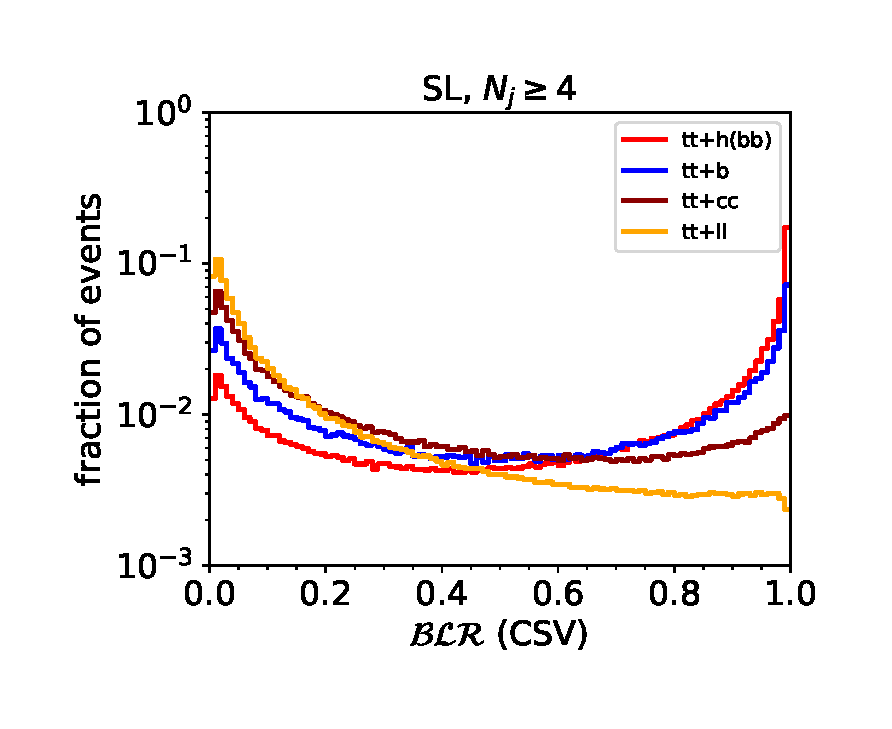
\includegraphics[width=0.5\textwidth]{figures/blr_shape_btagCSV.pdf}} 
\subfloat[Expected performance of the discriminant.]{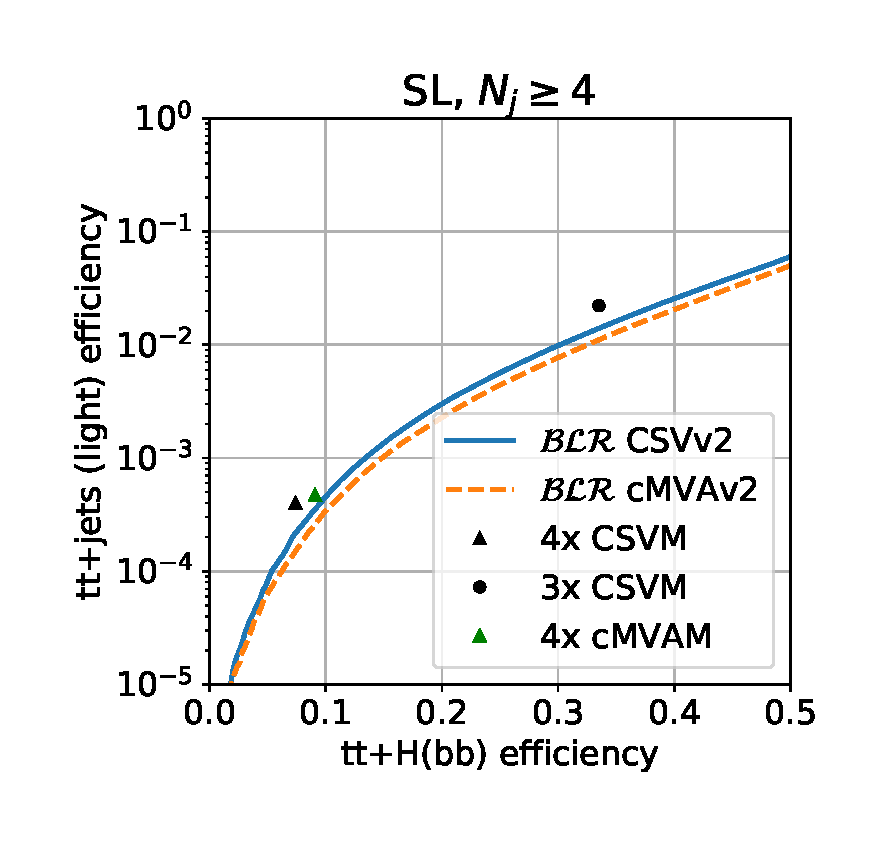
\includegraphics[width=0.5\textwidth]{figures/blr_roc.pdf}}\\
\caption[Expected performance of the b-tag likelihood ratio discriminant.]{Simulated distribution and expected performance of~$\mathcal{BLR}$~discriminant in the SL channel, requiring at least 4 good jets. On~(\textbf{a}), we show the simulated shapes of the discriminant for signal~(\ttHbb) and the various \ttbar+jets backgrounds. On~(\textbf{b}), we compare the efficiency to select~\ttHbb~and~\ttlf~events. We see that the~$\mathcal{BLR}$~discriminant compares favourably to a fixed cut on number of b tags. The~$\mathcal{BLR}$~ discriminator defined with the cMVAv2 b~tagger algorithm further improves the performance over the full range.}
\label{fig:blr_discrimination}
\end{centering}
\end{figure}


\begin{figure}
\begin{centering}
\subfloat[Fraction of events with correct matching.]{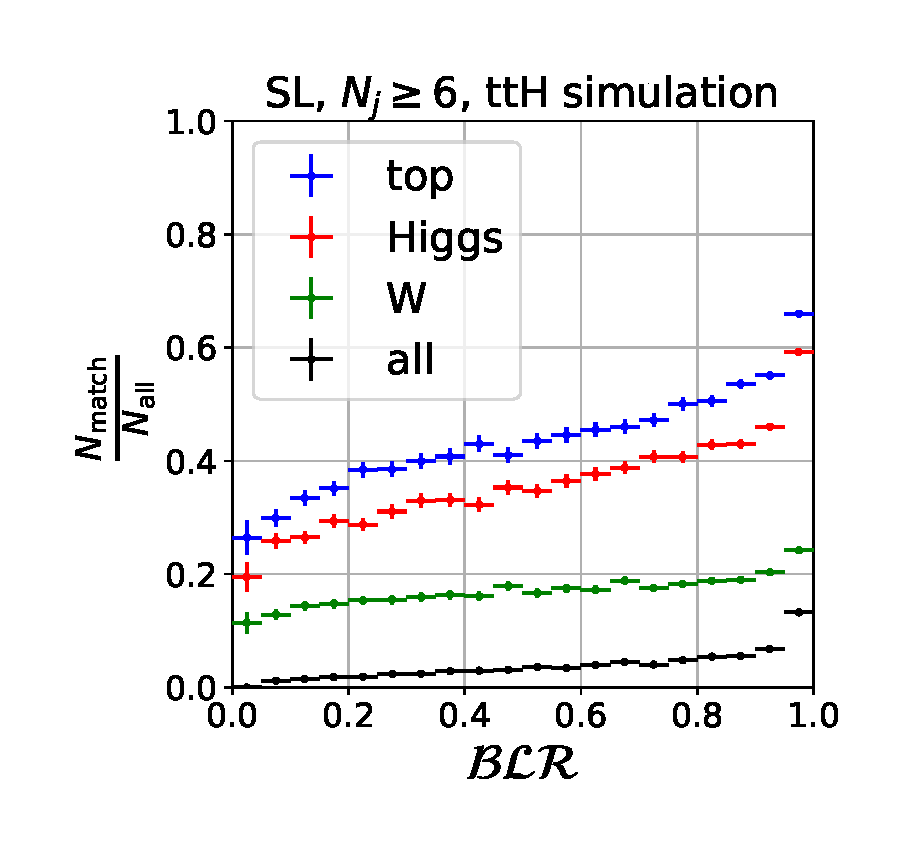
\includegraphics[width=0.5\textwidth]{figures/blr_matching.pdf}} 
\subfloat[Fraction of matched events with correct tagging.]{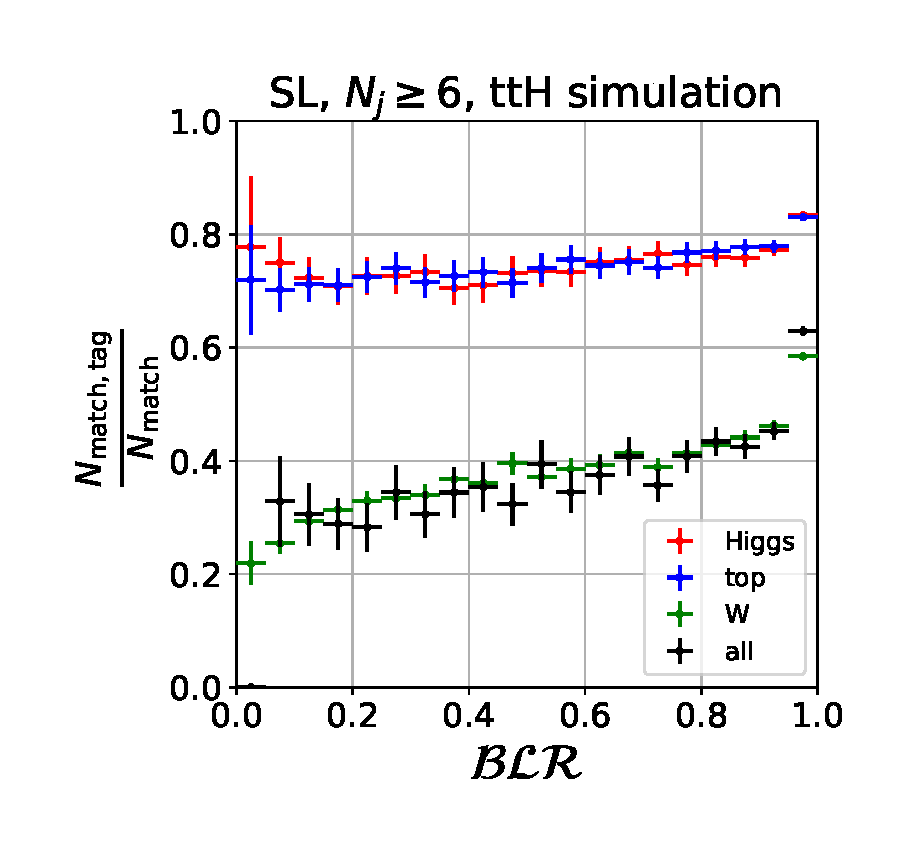
\includegraphics[width=0.5\textwidth]{figures/blr_matching_tag.pdf}}\\
\caption[Fraction of events with correct matching to the hard process]{Estimation of the fraction of events where the bottom quarks from the top quark, the Higgs boson and the light quarks from the W boson are reconstructed as jets in the final state on (\textbf{a}). We study the event-level b tagging efficiency on (\textbf{b}), where we plot the fraction of events where the highest-likelihood permutation correctly assigned the bottom quarks to jets with respect to all events where the quarks were reconstructed as jets without considering tagging.}
\label{fig:blr_matching}
\end{centering}
\end{figure}
 
The likelihood ratio as defined here ignores the differences in~$f(\xi_k | \mathrm{b})$~and~$f(\xi_k | \mathrm{c})$, meaning that in the case of~$\mathrm{W} \rightarrow \mathrm{c}\bar{\mathrm{s}} (\bar{\mathrm{d}})$~decays, the discriminator is suboptimal. We have investigated extending this likelihood to also account for the possibility of such decays by a straightforward extension of~$\mathcal{BL}(\vec{\xi} | M\mathrm{b}~1\mathrm{c})$. However, we have found that the additional combinatorial complexity suppresses any increased discrimination power and further progress in this would likely require methods that are better able to deal with the combinatorial problem using kinematic information.

We use this likelihood discriminant to define heavy-flavour enhanced regions, as well as to select the bottom quark candidates in the application of the MEM, as described in~\cref{sec:mem_application}. 

As we have used the detailed b tagging discriminator shape information in constructing the~$\mathcal{BLR}$, we must experimentally calibrate the full range of this observable using data. This is done by deriving a scale factor between data and simulation that depends on the discriminator value, jet kinematics and flavour using a tag-and-probe method. The tag jet is required to pass the medium operating point that has been described earlier and iteratively correcting the discriminator distribution of the probe jet. In order to extract the weight for the b jets, the procedure relies on dilepton~\ttbar~events with the contribution from light jets and backgrounds subtracted using simulation, whereas for the scale factor for light jets, Z+jets events are used. The procedure is iterative, as the scale factor for light jets is required for the extraction of the b jet scale factor and vice versa~\cite{CMS:2013sea,CMS-PAS-BTV-15-001}. The systematic uncertainties from this reweighting are described in~\cref{sec:systematic_unc}.

The leptonic decays of the W boson produce neutrinos, which are only partially reconstructed by the detector as \MET, defined as the negative sum of all the momenta of the reconstructed particles in the transverse plane. In the SL channel, we can directly associate the \MET with the transverse momenta of the neutrinos, through the modelling of the recoil as described in~\cref{sec:transfer_functions} whereas in the DL channel, only the total momentum of both neutrinosis  constrained by the \MET.

\section{Event selection and categorization}
\label{sec:event_selection}

First, the large multi-jet QCD background is reduced to negligible levels by requiring that at least one of the top quarks in \ttHbb decays leptonically. We divide events to two exclusive lepton categories: SL and DL, based on the multiplicity of the reconstructed charged leptons passing the quality cuts described in~\cref{sec:object_id_lep}. This is achieved by vetoing events with any additional leptons passing loosened quality criteria. For the dilepton category, we further suppress the Drell-Yan background by requiring~$m_{\ell\ell} > 20\GeV$~and Z+jets by rejecting events with~$76\GeV < m_{\ell\ell} < 106\GeV$. Furthermore, the leptons are required to have opposite charge. In the DL same-flavour channels, we require~$\MET > 40\GeV$. We do not explicitly distinguish between cases where the top quark decays to~$\mathrm{\tau}$~leptons, although these events can still pass the selection in case the~$\mathrm{\tau}$~decays leptonically.

Events from \ttHbb have a large number of jets and b tags compared to the V+jets backgrounds. Therefore, we require the presence of at least 4 jets passing the quality criteria (\cref{sec:object_id_jets}), out of which at least 2 must be b tagged according according to the medium working point (\cref{sec:object_id_btag}). This brings us to the~\ttbar~dominated region, where we further distinguish between 7 categories in the SL channel
\begin{itemize}
\item~$\ge 6~\mathrm{jets},\ge 4~\mathrm{b~tags}$;~$~5~\mathrm{jets},\ge 4~\mathrm{b~tags}$;~$~4~\mathrm{jets},4~\mathrm{b~tags}$, that are the most signal-enriched regions,
\item~$\ge 6~\mathrm{jets},3~\mathrm{b~tags}$;~$5~\mathrm{jets} 3,\mathrm{b~tags}$;~$5~\mathrm{jets},3~\mathrm{b~tags}$, that contain a significant amount of \ttcc and \ttbb,
\item~$\ge 6~\mathrm{jets},2~\mathrm{b~tags}$, that is \ttlf-enhanced and used to constrain JEC uncertainties,
\end{itemize}
and three categories in the DL channel
\begin{itemize}
\item~$\ge 4~\mathrm{jets},\ge 4~\mathrm{b~tags}$,
\item~$\ge 4~\mathrm{jets},3~\mathrm{b~tags}$,
\item~$~4~\mathrm{jets},2~\mathrm{b~tags}$,
\end{itemize}
resulting in a total of 10 exclusive categories.

We use the MEM as a \ttHbb to~\ttbb~discriminator in the categories with~$\ge 4$~b tags as these are the primary signal-enriched regions. The categories with 3 b tags ar further subdivided into~$\mathcal{BLR} \ge C$~(high) and~$\mathcal{BLR} < C$~(low), where the high categories are enriched in \ttHbb and therefore will rely on the MEM for discrimination. The low-$\mathcal{BLR}$~categories are retained as control regions where we fit the jet b tagging discriminator. In the categories with 2 b tags, we fit the jet~$p_T$~distribution in order to constrain the jet energy scale correction uncertainties. The value of~$C$~is determined so that it would result in a signal acceptance of~$\epsilon = 0.5$~and significantly lower background acceptance.

\section{Signal extraction}
\label{sec:mem_application}
The likelihood discriminant based on b tagging enhances the~\ttbar~+ heavy flavour component, but the cross-section of~\ttbb~is still an order of magnitude larger that \ttHbb. Furthermore, we cannot directly reconstruct the resonant peak of the \Hbb~decay as a natural disciminant between the signal and non-resonant background. Even though the width of the SM Higgs boson is relatively small compared to detector resolution ($\Gamma = X~\GeV$), the presence of multiple additional bottom quarks due to top decay in the final state creates a combinatorial self-background in the form of an ambiguity in choosing the candidate jets for the \Hbb~decay.

An experimental mass estimator built from randomly selected jet pairs results in a much broader distribution compared to experimental resolution, whereas choosing the pair of jets that would give a mass closest to~$m_H$~would cause also the background to exhibit a signal-like peak.

Therefore, we use the MEM discriminant, introduced in~\cref{sec:mem}, to compute theory-motivated weights~$P_{\ttHbb}$~and~$P_{\ttbb}$~for each candidate event. We construct a discriminant based on the likelihood ratio of these weights, as described in~\cref{sec:mem_performace}, which based on the Neyman-Pearson lemma, described in~\cref{sec:test_statistic}, is the optimal test statistic between the signal and background hypotheses.

As an improvement over the search for \ttHbb performed by the CMS experiment in Run I~\cite{Khachatryan:2015ila}, we use the MEM discriminant also in categories which are not fully reconstructed, but still contain a large amount of signal, namely 5-jet and 4-jet categories in the SL channel. The details of the additional MEM hypotheses are described in~\cref{sec:event_interpretation}. We list the discriminant that has been used in different categories in~\cref{tab:cat_discriminant}. 


\begin{table}[h!]
\begin{center}
\caption[The analysis categories for the~\ttHbb~analysis.]{The analysis categories and the discriminators used in those categories.}
\label{tab:cat_discriminant}
\begin{tabular}{c|c}
\hline
category & discriminant \\
\hline
SL~$\ge6$~jets,~$\ge4$~tags & MEM SL~$2_{\mathrm{W}} 2_{\mathrm{h}} 2_{\mathrm{t}}$~\\
SL~$\ge6$~jets,~$3$~tags & The b-tagging likelihood ratio~$\mathcal{BLR}$ \\
SL~$\ge6$~jets,~$2$~tags & leading jet~$p_T$~\\
\hline
SL~$5$~jets,~$\ge4$~tags & MEM SL~$1_{\mathrm{W}} 2_{\mathrm{h}} 2_{\mathrm{t}}$~\\
SL~$5$~jets,~$3$~tags,~$\mathcal{BLR}$~high & MEM SL~$1_{\mathrm{W}} 2_{\mathrm{h}} 2_{\mathrm{t}}$~\\
SL~$5$~jets,~$3$~tags,~$\mathcal{BLR}$~low & leading jet b discriminator \\
\hline
SL~$4$~jets,~$\ge4$~tags & MEM SL~$0_{\mathrm{W}} 2_{\mathrm{h}} 2_{\mathrm{t}}$~\\
SL~$4$~jets,~$3$~tags,~$\mathcal{BLR}$~high & MEM SL~$0_{\mathrm{W}} 2_{\mathrm{h}} 2_{\mathrm{t}}$~\\
SL~$4$~jets,~$3$~tags,~$\mathcal{BLR}$~low & leading jet b discriminator \\
\hline
DL~$4$~jets,~$\ge4$~tags & MEM DL~$2_{\mathrm{h}} 2_{\mathrm{t}}$~\\
DL~$4$~jets,~$3$~tags,~$\mathcal{BLR}$~high & MEM DL~$2_{\mathrm{h}} 2_{\mathrm{t}}$~\\
DL~$4$~jets,~$3$~tags,~$\mathcal{BLR}$~low & leading jet b discriminator \\
DL~$4$~jets,~$2$~tags & leading jet~$p_T$~\\
\hline
\hline
\end{tabular}
\end{center}
\end{table}

We use the~\ttbb~matrix element as a representative background in all cases. This gives the best separation in the most signal-rich categories against~\ttbb~and is further motivated by simulation, where we see that using this process as background still achieves a high rate of separation in categories enriched in other \ttbar+jets subprocesses. As a future improvement, considering additional background hypotheses in different categories is expected to improve the discrimination at the cost of computational complexity.

As the~$\mathcal{BLR}$~method is optimised to identify the set of jets that are most compatible with arising from 4 bottom quarks, we further augment the MEM by assuming that the bottom quarks need to be considered only among those 4 jets, as explained in~\cref{sec:event_interpretation}. This means that the we have exactly 4 candidates for the bottom quarks from \Hbb~and~$\mathrm{t} \rightarrow \mathrm{W} \mathrm{b}$~decay, whereas the remaining jets are assumed to arise from~$\mathrm{W} \rightarrow \mathrm{q} \mathrm{q}'$~or QCD radiation. 

In the next section, we will discuss the systematic uncertainties that affect the analysis.

\section{Systematic uncertainties}
\label{sec:systematic_unc}
We have already mentioned in passing that there are a number of experimental as well as theoretical uncertainties that must be taken into account.

Among the experimental uncertainties, the dominant ones are uncertainties on the jet energy scale corrections (\cref{sec:jec_unc}) and the reweighting of the b tagging discriminant (\cref{sec:btag_unc}). Both of these can affect the yields of all the processes, since they change the selection efficiency, as well as the shapes of the final discriminants. In case the source of the uncertainty is the same across several categories, the nuisance parameters associated with the uncertainties are treated as fully correlated.

From the theoretical uncertainties, the most important ones arise from the variation of the renormalization and factorization scale of the \ttbar+jets subprocesses and the \ttH signal. Furthermore, since the \ttbar+jets \texttt{POWHEG} model we currently use in the analysis treats the~\ttbb~process only at leading order accuracy, where the~$\mathrm{b}\bar{\mathrm{b}}$~pair is generated from gluon splittings using a parton shower, we have considerable additional theoretical uncertainties on the modelling of \ttbb.

We give a detailed overview of the most important experimental and theoretical uncertainties along with their estimation in the next sections. The full list of systematic uncertainties along with their effect is show in~\cref{tab:systematic_uncertainties}.

\begin{table}[h!]

\begin{center}
\caption{Systematic uncertainties in the~\ttHbb~analysis.}
\label{tab:systematic_uncertainties}
\begin{tabular}{c|cccc}
\hline
uncertainty & normalization & shape & process & model \\
\hline
JEC (26 sources) & yes & yes & all & gaussian \\
btag & yes & yes & all & gaussian \\
\hline
bla & yes & yes & all & gaussian \\
\hline
\hline
\end{tabular}
\end{center}
\end{table}

\subsection{Jet energy correction uncertainties}
\label{sec:jec_unc}
In Run II, we consider various sources of jet energy correction uncertainties with their corresponding correlations, as opposed to a single bulk JEC uncertainty as was done for this analysis in Run I. This significant advancement has resulted from an improved modelling of the detector performance and better calibration techniques developed with more data. 

The magnitude and correlation of the uncertainties on jet energy scale and resolution are estimated in a dedicated CMS analysis and are provided as a vector of per-jet corrections with~$p_T$~and~$\eta$~dependent correlations. The most important groups of correction uncertainties are the following.

\begin{itemize}
\item Pileup offset, which results from from extra energy deposited in jets from additional pp interactions within the same bunch crossing (in-time pileup) or due to the finite signal decay time in the calorimeters (out-of-time pileup). The uncertainty for this source results from the~$\eta$-dependent scale factor used to correct the offset distribution measured in simulation.
\item Relative~$\eta$-dependent corrections, which calibrate the forward regions of the detector with respect to the central region. The uncertainties on this source arise from jet energy resolution and from the modelling of ISR+FSR.
\item Uncertainties on the absolute energy scale, which are derived using Z/$\gamma$+jet and multijet data. The energy scale uncertainties are driven by the muon momentum scale and the single pion response in the HCAL. Furthermore, the uncertainties in fragmentation are assessed in a comparison of \texttt{PYTHIA} and \texttt{HERWIG++}.
\item Uncertainties in the modelling of the detector response for jet flavor, which are assessed using simulation and are largest for gluon jets.
\item Finally, due to radiation damage, there is a residual time-dependent uncertainty in the scale corrections, which is estimated using dijet events in different run periods.
\end{itemize}
These 5 groups factorize into about 26 independent sources with up and down variations.

In order to account for the JEC scale uncertainties in the analysis, we propagate the uncertainties in jet energy corrections and resolution to the jet momenta and all the event-level observables that derive from them in MC by shifting the jet energy scale by one standard deviation. This is done separately for all the sources so that we can fully account for the correlations between the various sources. Thus, we are able to account for both the changes in efficiency (normalization) and discriminator shape in the final analysis categories.
In order to propagate the uncertainty to a high-level multivariate observable such as the MEM, we need to recompute it using the variated objects. We use the approximate MEM variation technique of this as described in~\cref{sec:mem_uncertainties}.

In addition to uncertainties in the jet energy scale corrections, we also consider uncertainties on the jet energy resolution corrections. 
\subsection{B-tagging systematic uncertainties}
\label{sec:btag_unc}
Due to the high number of b tagged jets in the final state, this analysis is sensitive to uncertainties in b tagging. As we have described in~\cref{sec:object_id_btag}, we correct for mismodeling in the b tagging discriminator shape using a tag and probe method.

The uncertainties of this correction include the propagation of jet energy scale uncertainty, which affects the determination of the correction through changes in efficiency and the discriminator value. Furthermore, simulation is used to subtract the non-relevant jet flavor components in determining the scale factor for bottom (light) jets. For the scale factor for light jets, the fraction of bottom (charm) jets is variated within 20\% of the MC prediction in the Z+jets simulation used to determine the scale factors. Similarly, for the extraction of the b jet scale factor, the light flavour component in the \ttbar+jets dileptonic sample arises from additional radiation and is estimated to be 20\%~\cite{CMS-PAS-BTV-15-001}.

As the b discriminator scale factor is determined in bins of the discriminator value, statistical fluctuations in bins with a low number of data and simulated events introduce an uncertainty on the final scale factor. This uncertainty is only significant in case the size of the fluctuations varies systematically over the b discriminant range. Since the discriminator has a roughly monotonous increasing (decreasing) shape for b jets (light jets), this condition is fulfilled. The statistical uncertainties are accounted for by a sum of polynomials of first and second order, where the nuisance parameter is the overall scale of the distortion.

There is currently no dedicated scale factor for the b discriminator of charm jets, therefore, the uncertainty is conservatively assumed to be twice as large as for the b jet scale factor.

We propagate the uncertainties from b tagging in the form of a set of per-event weights, which are determined from the individual per-jet weights that are used to correct the jet b discriminator distributions.

\fixme plot of b-discriminator before and after re-weighting with shape uncertainties.

\subsection{Other systematic uncertainties}
We also assess the effect of uncertainties in the lepton identification, isolation and trigger selection, which may have different efficiencies in data and simulation and are thus corrected using scale factors. For muons, we assign a~$1\%$~normalization uncertainty for the lepton ID,~$1\%$~for isolation and~$0.5\%$~for the so-called HIP effect, on top of the statistical uncertainties on the muon scale factor\cite{CMS:2017_mu_sf}. For electrons, we use~$p_T$~and supercluster~$\eta$-dependent scale factor uncertainties derived using a tag-and-probe method, which are generally below~$1\%$~\cite{CMS:2017_ele_sf}.

As the pileup profile in simulation is corrected to data using a pileup-dependent scale factor, we estimate the uncertainty in the pileup correction by varying the minimum bias cross section from~$\sigma = 69.2$~mb by~$4.6\%$, corresponding to the uncertainty in the number of interactions in minimum bias events from luminosity and cross section\cite{CMS:2017_pu_weight_twiki}.

Furthermore, the uncertainty on total integrated luminosity is estimated to be~$2.5\%$~using cluster counting in the pixel detector and affects all processes\cite{CMS:2017sdi,CMS:2017_lumi}.

\subsection{Theoretical uncertainties}
The most important theoretical uncertainties arise from the \ttbar+heavy flavour processes, namely \ttbb, \tttwob, \ttb~and \ttcc. Currently, there is no direct way to determine these backgrounds directly from data. Therefore, we assign a conservative 50\% normalization uncertainty on all the \ttbar+heavy flavour processes, uncorrelated across the aforementioned subprocesses.

The cross sections of all involved signal and background processes are known to at least NLO accuracy, with uncertainties estimated through PDF QCD renormalization and factorization scale variations on the \ttbar~background. Furthermore, we use dedicated MC simulation to estimate the effect of the renormalization and factorization scales and the initial and final state radiation on the final discriminant shape. Shape uncertainties from PDF variations are found to be negligible and thus not considered further in the analysis.

\section{Statistical method}
\label{sec:statistical_method}
In order to interpret the data, we use the same statistical framework as has been used for other Higgs boson searches in the CMS collaboration\cite{Chatrchyan:2012xdj,Chatrchyan:2012tx,ATLAS:2011tau}. We wish to measure the signal strength modifier~$\mu = \sigma_{\ttH}/\sigma_{\ttH,\mathrm{SM}}$~and in the absence of an observed signal, exclude~$\mu \ge \mu^{CL}$~at a certain confidence level. The null hypothesis ($H_0$) is therefore the presence signal with a given~$\mu$~and background, whereas the alternative hypothesis is no signal ($H_1, \mu = 0~$). Based on the data, we seek to exclude the null hypothesis above a certain~$\mu$.

The predictions for both signal (denoted as~$s$) and background (denoted as~$b$) yields are subject to uncertainties introduced in~\cref{sec:systematic_unc} such that the expectations are functions of the nuisance parameters~$\theta$:~$s(\theta)$~and~$b(\theta)$. The uncertainties are assumed to be either fully correlated or uncorrelated, as is more appropriate and conservative, which allows the likelihood function to be written in a factorized form.

To determine confidence intervals on the Higgs boson production cross section and thus quantify the absence of a signal, we use the~$CL_s$~method~\cite{Junk:1999kv,Read:2002}, which defines the likelihood function~$\mathcal{L}(\mathrm{data} | \mu, \theta)$~as

\begin{align}
\label{eq:likelihood}
\mathcal{L}(\mathrm{data} | \mu, \theta) =&  \mathrm{Poisson}(\mathrm{data} | \mu \cdot s(\theta) + b(\theta)) \cdot p(\tilde{\theta} | \theta)\\
=& \prod_{i\in \mathrm{bins}} \frac{(\mu s_i + b_i)^{n_i}}{n_i!} \exp{[-(\mu s_i + b_i)]} \cdot p(\tilde{\theta} | \theta).
\end{align}
We have used Poisson probabilities to model the observation of~$n_i$~events in the bin~$i$~of a discretized distribution, given an expectation~$\mu s_i + b_i$. The distribution~$p(\tilde{\theta} | \theta)$~encodes the prior knowledge on the nuisance parameters, which have default values~$\tilde{\theta}$. This likelihood function can be computed both with observed data and with "pseudo-data", which is constructed from simulation under a specific hypothesis.

We use the test statistic~$\tilde{q}_\mu$, based on the profile likelihood ratio\cite{Cowan:2010js}, to assess the compatibility of the data with either the \textit{background-only} or \textit{signal+background} hypotheses:

\begin{equation}
\tilde{q}_\mu = -2 \ln{\frac{\mathcal{L}(\mathrm{data} | \mu, \hat{\theta}_\mu)}{\mathcal{L}(\mathrm{data} | \hat{\mu}, \hat{\theta})}},\ 0 \le \hat{\mu} \le \mu.
\end{equation}
This test statistic is constructed such that it considers only models with~$\mu \ge 0$, furthermore it is constrained to be one sided by~$\hat{\mu} \le \mu$~such that data with~$\hat{\mu} > \mu$~are not used as part of the rejection region for the test on the upper limit of~$\mu$.

Here~$\hat{\theta}_\mu$~is the conditional maximum likelihood estimator of~$\theta$~given a fixed value~$\mu$, whereas~$\hat{\mu}$~and~$\hat{\theta}$~refer to the overall maximum likelihood estimators of both quantities. For a given signal strength modifier~$\mu$~that we test, we first find the observed value of~$\tilde{q}_\mu^{\mathrm{obs}}$~and the nuisance parameters~$\hat{\theta}_0$~(background hypothesis) and~$\hat{\theta}_\mu$~(signal hypothesis). Then, in order to compute the~$\mathrm{CL}_s(\mu)$, we compute the p-values of the signal and background hypotheses using

\begin{equation}
p_{\mu} = \int_{\tilde{q}_{\mu}{\mathrm{obs}}}^\infty f(\tilde{q}_{\mu} | \mu, \hat{\theta}_{\mu})\ \mathrm{d}\tilde{q}_\mu
\end{equation}
and

\begin{equation}
1 - p_b = \int_{\tilde{q}_{\mu}^{\mathrm{obs}}}^\infty f(\tilde{q}_{\mu} | 0, \hat{\theta}_0)\ \mathrm{d}\tilde{q}_{\mu}.
\end{equation}

The p-values are the probabilities of observing results as extreme or more given the underlying hypothesis and are derived from the probability densities of~$\tilde{q}_{\mu}$~under a given hypothesis:~$f(\tilde{q}_\mu | \mu, \hat{\theta}_\mu^{\mathrm{obs}})$. We find the 95\% confidence level on the upper limit of~$\mu$~by adjusting~$\mu$~until

\begin{equation}
\mathrm{CL}_s(\mu) = \frac{p_\mu}{1 - p_b} < 0.05.
\end{equation}
Equivalently, if~$\mathrm{CL}_s < \alpha$~at~a given $\mu$, then the Higgs boson is excluded at a production rate of~$\mu$~or higher with a confidence level~$1 - \alpha$.

In order to compute the upper limit on~$\mu$~given the observed data, we need the PDFs~$f(\tilde{q}_\mu | \mu, \hat{\theta}_\mu^{\mathrm{obs}})$, which can be derived using a Monte Carlo method by generating pseudo-data assuming the given signal strength~$\mu$~and fitting the observed data to evaluate the test statistic. As the MC procedure for generating the PDFs can be very time consuming, we use an approximate asymptotic distribution~\cite{Cowan:2010js} for the PDF~$\tilde{q}_\mu$, which results from the Wald approximation~\cite{wald1943tests}:

\begin{equation}
-2 \ln{\lambda(\mu)} = \frac{(\mu - \hat{\mu})^2}{\sigma^2}+ \mathcal{O}(1/\sqrt{N})
\end{equation}
where~$\sigma$~is the standard deviation of~$\hat{\mu}$~derived from the full covariance matrix of the likelihood function.

Using the asymptotic distribution for~$f(\tilde{q}_\mu | \mu, \hat{\theta}_\mu^{\mathrm{obs}})$, we find the upper limit for~$\mu$~at a confidence level of~$1 - \alpha$~to be

\begin{equation}
\mu = \hat{\mu} + \sigma \Phi^{-1}(1 - \alpha)
\end{equation}
where~$\Phi^{-1}$~is the inverse of the cumulative distribution of the Gaussian PDF. The standard deviation of~$\mu$~can be computed from the likelihood function~\cref{eq:likelihood} using the so-called Asimov data set, where the MC prediction is used for~$s_i$~and~$b_i$.

We will also quote the expected sensitivity of the measurement, which is derived from simulation, assuming~$\mu = 1$~and computing the median expected upper limit on~$\mu$~using the asymptotic formulae. 

\subsection{Uncertainties in the statistical model}

Our prior knowledge of the systematic uncertainties is encoded in~$p(\tilde{\theta} | \theta)$, where the nuisance parameters~$\theta$~are minimized in the profile likelihood method in a frequentist sense. We use~$\tilde{\theta}$~to represent our best estimate of the nuisance parameters, which can be
\begin{itemize}
\item Gaussian, used for shape variations,
\item log-normal used for nuisances that do not have physical negative values,
\item flat, in case we cannot assign a prior uncertainty.
\end{itemize}

We use the Barlow-Beeston method in the fit to account for limited number of simulation events. In this method, the number of predicted events for a background component in a binned distribution is added as a nuisance parameter in the likelihood and minimized with the initial values arising from the observed Poisson counts using Newton's method~\cite{Barlow:1993dm}. 

\subsection{Analysis of the model}
In this section, we will study the expected sensitivity predicted by the statistical model. We will look in detail at the effect of systematic uncertainties in the form of the constraints on the nuisance parameters after having been fit to pseudo-data derived from MC.

\section{Results}
After having validated the statistical model on simulation, we include data in a step-by-step fashion by unblinding the data in the various control regions successively.
